\chapter{Evaluation}

The two algorithms from Chapter~\ref{ch:dynprog} and Chapter~\ref{ch:heuristic} both decide Problem~\ref{prob:weak-udc-lobster} for size $n$ lobsters in time linear in $n$. In this chapter, we extend our understanding of their performance and correctness in practical application.

We provide a software implementation of the approaches. Then we measure the run time and answers on the exhaustively enumerated set of all lobster instances with spine length ranging from 2 to 7.

\section{Software Implementation}

Both algorithms are included in the functionality of the \texttt{udcrgen} (``unit disk contact representation generator'') program, which was entirely written as part of this thesis. \texttt{udcrgen} is written in C++ using the standard library and no other dependencies---though its unit tests do depend on Google Test~\cite{GoogleTest}. It uses the CMake~\cite{CMake} build system. The source code is available online.\footnote{\url{https://git.ac.tuwien.ac.at/soeren.nickel/peter_neubauer.git}}.

The program reads in a graph instance, runs one of the available algorithms on it and produces statistical output. This output contains, for every instance tested, the algorithm used, the instance size, spine count, recognition success (yes/no) and runtime. \soeren{What does statistical output mean here?}\peter{added details} If the instance is found to admit an embedding, \texttt{udcrgen} can also output such an embedding as a drawing.

It additionally offers ``benchmark mode'', in which it does not read an instance as input. Instead, it generates an enumeration of possible lobsters within user-specified restrictions on spine count given as input parameters. All generated instances become inputs for the algorithms. Though the enumeration omits some instances to save time, it covers enough to decide any lobster within the given limits. We describe the exact method in Section~\ref{section:ch6-enumeration} below. \soeren{What kind of equivalence? Maybe up to isomoprphism?}\peter{reformulated}

During execution, \texttt{udcrgen} produces diagnostic log messages at different levels of detail. The level and target log file can be configured by the user.

These algorithms are implemented in the program:

\begin{itemize}
    \item The ``strict contact'' algorithm described by Klemz et al.~\cite{Klemz2015}, with a configurable gap size for minimum distance of disks not in contact. It applies only to caterpillar graphs.
    \item The ``dynamic program'' described in Chapter~\ref{ch:dynprog}.
    \item The ``heuristic algorithm'' described in Chapter~\ref{ch:heuristic}. It features an ``embed order'' parameter, which selects either the depth-first or breadth-first order of vertices.
\end{itemize}

Input graphs may be given (if not generated) either

\begin{itemize}
    \item in a \emph{degree notation}---see Section~\ref{section:ch6-enumeration}---, which specifies the vertex degree of each spine vertex in a caterpillar, or
    \item as an \emph{edge list}, which may describe any graph. The program recognizes a caterpillar or lobster, if possible, and converts it to an internal representation as described in Section~\ref{section:ch6-graph-representation}. If provided with an unrecognized type of graph, the program terminates with an error.
\end{itemize}

The decision result and runtime measurement are recorded in a CSV file. The drawing(s) of yes-instances may be written to an \texttt{.ipe} file, the format of the IPE drawing editor~\cite{cheong_ipe_2022} (only in a single-instance mode), or in SVG format to an HTML file (also in benchmark mode).

\texttt{udcrgen} can also create an \emph{archive} consisting of two directories: one to hold all the yes-instances encountered, and another one for the no-instances. The archive uses a degree list format.

\section{Instance Enumeration}
\label{section:ch6-enumeration}

To exhaustively examine lobsters with $n$ spine vertices, we must define a systematic method of enumerating them. Our idea is based on the degree notation for lobsters. In this notation, a lobster with $n$ spine vertices is represented as an \emph{identifier} string $$d_{1,1}d_{1,2}d_{1,3}d_{1,4}d_{1,5}\_d_{2,1}d_{2,2}d_{2,3}d_{2,4}d_{2,5}\_\ldots\_d_{n,1}d_{n,2}d_{n,3}d_{n,4}d_{n,5},$$ where $d_{i,j} \in \{ \texttt x, 0, 1, 2, 3, 4, 5 \}$ is the number of leaf vertices adjacent to the $j$th branch on the $i$th spine vertex, or $\texttt x$ to signify ``no branch at this index''. We consider the $\texttt x$ equivalent to $-1$ for ordering purposes.
Any lobster instances with $n \geq 2$ that contain too many branches or leaves to be represented in this way certainly do not admit a disk contact embedding.\soeren[inline]{I'm not sure what the last sentence points out. Why is this specific to $n\leq 2$?}\peter[inline]{A single spine vertex is the only case that fits 6 branches. Should I add a comment to that effect?}

For all $1 \leq i \leq n, 1 \leq j \leq 5$ we initialize $d_{i,j} = \texttt x$, starting with a lobster consisting only of a spine without any branches. We instantiate the internal graph representation from the degree notation and test it with regards to the decision problem.
We obtain the next identifier by interpreting it like a $5n$-digit base-7 number, which we increment. If the last digit overflows, we carry the increment to the next digit and so on.

\begin{table}
\centering
\begin{tabular}{ r|r|r|r }
\toprule
Spine Length & Yes-Instances & No-Instances & Max. Vertex Count (Yes) \\
 \hline
2	 & 141	 	& 101 	& 24 \\
3	 & 1107	 	& 757 	& 29 \\
4	 & 9343	 	& 6297 	& 34 \\
5	 & 80952	& 54336 	& 39 \\
6	 & 698352	& 468667 	& 44 \\
7	 & 6041183	& 4053036 	& 49 \\
\bottomrule
\end{tabular}
 \caption{Through our enumeration, we discovered the listed number of lobsters. This enumeration is exhaustive for the given sizes, meaning that it accounts for every yes-instance for Problem~\ref{prob:weak-udc-lobster} up to efficient omissions by branch order, orientation and dominance discussed in this chapter. The no-instances are not exhaustive. They are simply informative about the arbitrary number of data points which emerged from our method of ``adding vertices until it fails''. This even lead us to evaluate lobsters with one more vertex than the ``maximum'', which naturally all fail quickly due to insufficient space. }
\label{tbl:instance-count}
\end{table}

By this naive method, the number of tests to run for size $n$ is $7^{5n}$. The actual number of instances which we evaluated in practice is listed in Table~\ref{tbl:instance-count}. We reduce the necessary work in several ways.

\subsection{Branch Ordering}

Since the minimum distance from a spine vertex is by definition the only distinguishing feature for any vertex in a lobster, we can always exchange any two branches of the same spine by swapping $d_{i,j}$ and $d_{i,k}$ in the representation. It still identifies the same lobster.
% We therefore define that $\texttt x < 0$
\soeren{For this purpose, you could define \texttt{x} as $-1$ in the thesis, even though the actual format is using \texttt{x}. This discrepancy can be specified in the definition.}\peter{done} We constrain our representation with the following \emph{branch ordering criterium}:

$$d_{i,j} \leq d_{i,k} \text{ if } j < k.$$

This reduces the valid representations to $\binom{7 + 5 - 1}{5}^n = 462^n,$ where $\binom{7 + 5 - 1}{5}$ is the number of 5-multisets from 7 elements.

\subsection{Orientation}

Let $s_1,\ldots,s_n$ be the sequence of spine sections---5 digits each. The sequence $s_n,\ldots,s_1$ then identifies the same lobster. We remove these duplicates from consideration by defining some arbitrary order $<_s$ over all valid spine constellations and enforce that the spine sequence must be \emph{canonically oriented}. A sequence has canonical orientation if

\begin{itemize}
    \item it is the empty sequence or
    \item $s_1 <_s s_n$ or
    \item $s_1 = s_n$ and $s_2, \ldots, s_{n-1}$ is canonically oriented.
\end{itemize}
%\soeren[inline]{Does this effectively half the number of considered sequences? Or can we make another statement about the effect on the number of considered instances.}
%\peter[inline]{Almost half (palindromes)}

\subsection{Dominance}

Let $$A = a_{1,1}a_{1,2}a_{1,3}a_{1,4}a_{1,5}\_\ldots\_a_{n,1}a_{n,2}a_{n,3}a_{n,4}a_{n,5}$$ and $$B = b_{1,1}b_{1,2}b_{1,3}b_{1,4}b_{1,5}\_\ldots\_b_{n,1}b_{n,2}b_{n,3}b_{n,4}b_{n,5}$$ be two lobster identifiers. Then $A$ \emph{dominates} $B$ if for all $1 \leq i \leq n, 1 \leq j \leq 5, a_{i,j} \leq b_{i,j}$. Since $A$ is easier than $B$, if we determine that $A$ does not admit an embedding, we infer that $B$ does not admit an embedding either and forgo testing the lobster described by $B$.

Similarly, if we would first determine that $B$ does admit an embedding, we may conclude that $A$ does as well. In practice, this does not help us because we examine our lobsters in strict incremental order.
%As an aside, note that this property might theoretically be exploited better by considering the set of spine constellations as a poset and locating the frontier of disk contact lobsters by binary search methods.
\soeren{Do you have a reference for binary search methods on posets?}\peter{No. Better drop the ``aside''.}

\subsection{Heuristic-Based Skip}

The test on any given lobster may, depending on the user's choice, involve running both the heuristic algorithm and the dynamic program. If this is the case, and if we are only interested in learning the answer to the decision problem (not in comparing the performance of the algorithms), then the fast heuristic solution should be attempted first. If it succeeds in finding that the input is a disk contact lobster, the slower exact algorithm can be skipped.

Our experiment, described below in Section~\ref{section:ch6-experiment}, does in fact compare algorithm performance. Thus we do not apply this particular optimization.

\section{Graph Representation}
\label{section:ch6-graph-representation}

The internal graph representation is the data structure which our algorithms operate on when they answer the disk contact problem. It must fulfill the following design criteria.

\begin{itemize}
    \item Sparsity---the structure should not store more than $O(n)$ data points for $n$ vertices.
    \item Fast traversal must be supported under admissible depth-first and breadth-first orders as defined in Chapter~\ref{ch:dynprog} and Chapter~\ref{ch:heuristic}.
    \item The query of relevant vertex properties must be fast:
    \begin{itemize}
        \item the depth of the vertex---0 for spines, 1 for branches and 2 for leaves and
        \item the number of children, i.e. vertices which have the queried vertex as their parent.
    \end{itemize}
    \item The internal representation must be easily convertible from the (user-supplied and generated) input graph formats as well as to the supported embedding output formats.
\end{itemize}

\begin{figure}
    \centering
    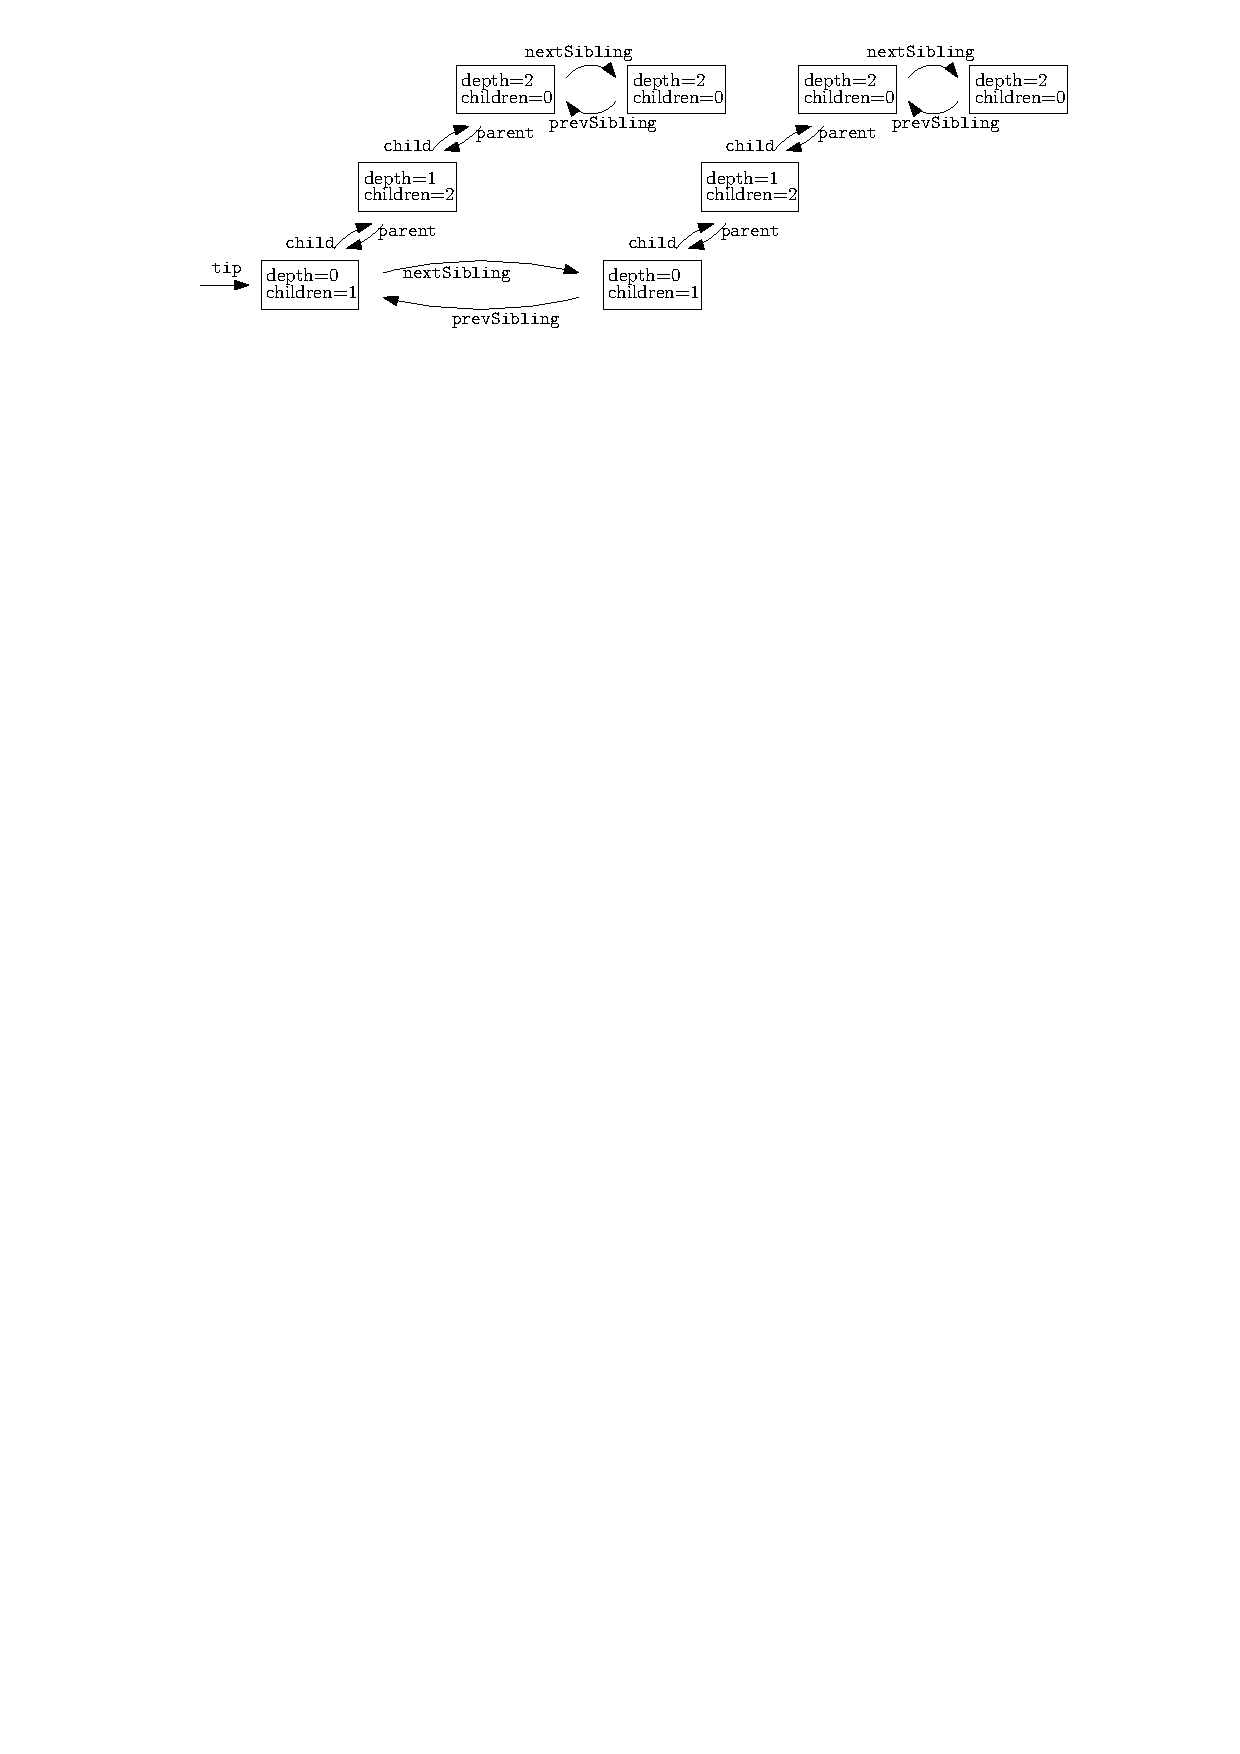
\includegraphics{graphics/ch6_diskgraph.pdf}
    \caption{The \texttt{DiskGraph} data structure with \texttt{Disk}s.}
    \label{fig:ch6_diskgraph}
\end{figure}

In the implementation, this structure is named \texttt{DiskGraph}. It holds a collection of \texttt{Disk}s and a pointer to the \texttt{tip}, which is the \texttt{Disk} that represents the first spine vertex. The \texttt{Disk} structure holds the vertex properties, including the constructed result of the (partial) embedding of that vertex. Figure~\ref{fig:ch6_diskgraph} illustrates the structure. \texttt{Disks} are represented by boxes and pointers by arrows.

\subsection{Format Conversion}

To convert from and to the degree list representations to the internal representation and also to produce the drawing from the coordinate data is trivial. However, the implementation can also accept an input graph as an edge list, which can describe any graph. In that case, we remove all the leaves to see if there remains just a string of vertices. If so, the graph is a caterpillar. Otherwise, we again remove all the leaves from the remainder to see if there remains just a string of vertices. If so, the graph is a lobster. We can reconstruct the removed graph components in reverse order.

These steps run in time $O(n)$ for $n$ input edges.
\soeren[inline]{I am not sure if we need this procedure in this detail. It kinda follows from the caterpillar definition. Let's discuss on Tuesday.}\peter[inline]{shortened}

\section{Experiment}
\label{section:ch6-experiment}

We ran the \texttt{udcrgen} software in benchmark mode with the dynamic programming algorithm, the heuristic algorithm with depth-first order and the heuristic algorithm with breadth-first order. The hardware specifications of the university-scale system used were: CPU: 2× Intel Xeon E5-2630 v2, 2.60GHz 6-core, RAM: 48GB.\soeren{This sentence is mssing something}\peter{better?} Note that the implementation is not parallelized.

The benchmark covers lobsters with at least $2$ and at most $7$ spine vertices enumerated using the scheme described in Section~\ref{section:ch6-enumeration}. In total, $11,414,272$ lobsters were evaluated.

\subsection{Dynamic Program Runtime}

\begin{figure}
    \centering % used for centering Figure
    \scalebox{1}{\includestandalone[]{standalone/runtime-dp}}
    \scalebox{1}{\includestandalone[]{standalone/runtime-dpyes}}
    \ref{legend:runtime-dp}
%     \centering
% \begin{tabular}{cc}
%     \includestandalone[]{standalone/runtime-dp} & \multirow{2}*{AAA\ref{legend:runtime-dp}} \\
%     \scalebox{1}{\includestandalone[]{standalone/runtime-dpyes}} & \\
% \end{tabular}
    \caption{The runtime of the dynamic program is depicted here. Every plotted point indicates the mean across all data points from the experiment with the same vertex count, spine length and instance class. Marks are colored and shaped according to the spine length and instance class. The second plot holds the same data, illustrating just the yes-instances.}
    \label{fig:ch5_runtime_dp}
\end{figure}

\begin{table}[t]
\centering
\begin{tabular}{ r|r|r|r|r|r|r }
\toprule
 $|V|$ & \#yes & \#no & $\varnothing \mu s$ DP/yes & $\varnothing \mu s$ DP/no & $\varnothing \mu s$ H/yes & $\varnothing \mu s$ H/no \\
 \hline
3	& 2 		& 0     	& 4.50		& 			& 6.50	&       \\
9	& 130		& 3     	& 30.55		& 80.75		& 18.49	& 15.50 \\
15	& 3272		& 385   	& 79.59		& 571.58	& 33.68	& 33.55 \\
21	& 31581		& 7028  	& 198.35	& 2,339.30	& 28.32	& 28.08 \\
27	& 151315	& 47442		& 396.52	& 4,428.87	& 39.14	& 38.48 \\
33	& 351093	& 157841	& 785.80	& 6,915.08	& 42.01	& 41.63 \\
39	& 402216	& 290471	& 1,414.34	& 9,979.08	& 51.02	& 49.88 \\
45	& 203481	& 251466	& 1,992.04	& 14,865.16	& 58.65	& 55.72 \\
\bottomrule
\end{tabular}
\caption{This excerpt of the experiment data shows the mean runtime of the dynamic program (under ``DP'') next to the heuristic with DFS order (under ``H''). The data is aggregated from all instances of the specified vertex count $|V|$ and class as specified in the header (``yes''/``no''). The number of data points aggregated in the ``DP'' columns is the same as the number of yes- and no-instances (``\#yes'', ``\#no'').}
\label{tbl:runtime}
\end{table}

In Figure~\ref{fig:ch5_runtime_dp} and Table~\ref{tbl:runtime}, we see the resulting average execution time of the dynamic program on lobsters of different sizes.

Among same-sized instances, those with a longer spine run faster. This is because there are fewer candidate coordinates for a spine vertex than for a branch vertex, and fewer candidates for a branch than a leaf.

We can observe that starting from about 25 vertices, the runtime of the dynamic programming algorithm is linear in the size of the input. The reason for the sharper rise in smaller instances, especially among yes-instances, is that the proportion of leaf vertices, which cause the greatest number of sub-problems to consider, grows initially and later remains constant in longer lobsters.

No-instances in our benchmark generally take far longer to compute than yes-instances. One reason is the early exit strategy discussed in Section~\ref{section:ch3_earlyexit}, which allows yes-instances to be answered without evaluating many of the generated sub-problems. Another reason is the way we enumerate instances, described above in Section~\ref{section:ch6-enumeration}. All our no-instances are at the brink of being ``almost solvable''. With these instances, we rarely encounter an early clog of too many vertices which would refute the instance. The algorithm is really forced to exhaust every possibility.

\subsection{Heuristic Runtime}

\begin{figure}[t]
    %\setlength{\unitlength}{0.14in} % selecting unit length
    \centering % used for centering Figure
    \scalebox{1}{\includestandalone[]{standalone/runtime-heuristic-dfs}}
    \scalebox{1}{\includestandalone[]{standalone/runtime-heuristic-bfs}}
    \ref{legend:runtime-heuristic}
    \caption{The runtime of the heuristic is depicted here both for depth-first and breadth-first order. Every plotted point indicates the mean across all data points from the experiment with the same vertex count, spine length and instance class. Marks are colored and shaped according to the spine length and instance class.}
    \label{fig:ch5_runtime_heuristic}
\end{figure}

\soeren[inline]{These figures are nice (although we need to change some things about the vertical axis labeling and maybe we can add a figure which puts the runtimes in relation to each other), but we need more explanation, both in the text and in the caption. Also we should discuss the consistent but discrete jumps at 19, 25, 32 and so on. Finally I think in particular to explain the jumps, the order in which things were ran on the cluster might actually be helpful here. Definitively we should discuss this on Tuesday.}

\begin{figure}
    %\setlength{\unitlength}{0.14in} % selecting unit length
    \centering % used for centering Figure
    \scalebox{1}{\includestandalone[]{standalone/runtime-dp-vs-h}}
    \caption{This is a direct comparison of the mean runtime of the dynamic program and the heuristic with DFS order. The scale is logarithmic, as at linear scale, the heuristic runtime simply appears flat at the bottom. Marks are colored and shaped by algorithm and instance class.}
    \label{fig:ch6-runtime-dp-vs-h}
\end{figure}
\peter[inline]{Neue Figure: Vergleich Heuristic vs Dynamic Prog (runtime)}

Figure~\ref{fig:ch5_runtime_heuristic} and Table~\ref{tbl:runtime} show the empirical runtime of the heuristic algorithm tested on the same set of instances as the dynamic program.

The same data in direct comparison with the dynamic program data is shown in Figure~\ref{fig:ch6-runtime-dp-vs-h}.

Overall, the heuristic offers up to about a $30\times$ speedup compared to the dynamic program on similar-sized yes-instances and about $250\times$ speedup compared to the dynamic program on our no-instances---which are, as mentioned before, generally unfavorable to the dynamic program.

While the dynamic program is faster on instances with more spines, the heuristic algorithm seems to require a small, fairly constant amount more time to place a spine in our implementation. The trend is linear in the vertex count of the instance, as expected. There is no performance difference between yes- and no-instances.

The consistent sudden increase in runtime around specific vertex counts, especially $15$ and $31$, are not related to any feature of the problem instances. Instead, they can probably be attributed to quirks of the \texttt{std::unordered\_map} associative data structure from the C++ standard library implementation used on the test system. This container holds the vertex coordinates in our heuristic algorithm implementation. The system used for the full experiment used GNU \texttt{libstdc++}, while the alternative experiment (on lobsters of spine length 2--4) depicted in Figure~\ref{fig:ch6-runtime-heuristic-alternative} ran on a Windows system using Microsoft's C++ standard library implementation. The alternative experiment does not show the same pattern of ``jumps''.

\begin{figure}
    %\setlength{\unitlength}{0.14in} % selecting unit length
    \centering % used for centering Figure
    \scalebox{1}{\includestandalone[]{standalone/runtime-heuristic-dfs-alternative}}
    \scalebox{1}{\includestandalone[]{standalone/runtime-heuristic-bfs-alternative}}
    \ref{legend:runtime-heuristic-alternative}
    \caption{The runtime of the heuristic as in Figure~\ref{fig:ch5_runtime_heuristic}, sampled on a different system for comparison.}
    \label{fig:ch6-runtime-heuristic-alternative}
\end{figure}

\subsection{Heuristic Accuracy}

\begin{figure}
    %\setlength{\unitlength}{0.14in} % selecting unit length
    \centering % used for centering Figure
    \scalebox{.8}{\includestandalone[]{standalone/accuracy}}
    \caption{The circles indicate the percentage of yes-instances correctly recognized by the two variations of the heuristic algorithm.}
    \label{fig:ch5_accuracy}
\end{figure}

\begin{table}
\centering
\begin{tabular}{ r|r|r|r|r }
\toprule
Spine Length & Yes-Instances & No-Instances & Yes (DFS) & Yes (BFS) \\
\hline
2	& 141	& 101			& 126	  (89\%) & 93      (66\%) \\
3	& 1107	& 757			& 1023	  (92\%) & 778     (70\%) \\
4	& 9343	& 6297			& 8092	  (87\%) & 6077    (65\%) \\
5	& 80952	& 54336			& 65635	  (81\%) & 48652   (60\%) \\
6	& 698352	& 468667	& 529979  (76\%) & 387235  (55\%) \\
7	& 6041183	& 4053036	& 4285811 (71\%) & 3090527 (51\%) \\
\bottomrule
\end{tabular}
\caption{Listing of the number of lobsters evaluated in the experiment, summed by spine length. The columns ``Yes (DFS)'' and ``Yes (BFS)'' show the absolute and relative number of lobsters which we know to be yes-instances (verified by the dynamic program) recognized as such by the heuristic using the indicated vertex order.}
\label{tbl:heuristic-accuracy}
\end{table}

Our heuristic approach with depth-first order answers between $70\%$--$90\%$ of all yes-instances of spine length 2--7 correctly. Figure~\ref{fig:ch5_accuracy} shows the percentages for the depth-first vertex order in red and compares it to the breadth-first variant in blue. The variant is shown to perform consistently worse by around $20$ percentage points.
\soeren[inline]{One final table giving the exact percentages and maybe the instance count would be nice here. Although we might want to include the instance count in the earlier suggested table.}
